\chapter{Smith-Whitten Coordinates}\label{smith}
\section{Coordinate Mapping}\label{Appendix_2_1}
Johnson has given a detailed description of how the three-body system can be represented in a symmetric way \cite{Johnson1980}. In this section we present the main procedures used to retrieve a mapping for the three-dimensional triatomic potential energy surface to a point in configuration space. This mapping will treat the different arrangement channels equally, which enables permutation symmetries for three identical particles to be imposed exactly. Performing a second mapping of the original representation presented in \cite{Smith1962,Smith_Whitten1968} yields the resulting set of modified Smith-Whitten coordinates. The derivation of the Hamiltonian for this representation is then described in \cref{Appendix_2_2}. Some of the definitions presented in \cref{MNJC} will be repeated here in oredr for this appendix to be complete.

Let $\mathbf{x}_i$ and $m_{i}$ be the position vector and mass of the $i$th particle in the laboratory frame. If the total mass $M$, the three particle reduced mass $\mu$, and the normalizing constants $d_{k}$ $(k=1,2,3)$ are given by

\begin{align}
M &= \sum_{i=1}^{3}m_i, \\
\mu^2 &= \prod_{i=1}^{3}m_i/M,\\
d_k^2 &= \frac{m_k}{\mu}\frac{(m_i+m_j)}{M},
\end{align}
then the set of mass-scaled Jacobi vectors and the center of mass coordinate can be defined as

\begin{align}
\mathbf{r}_k &= d^{-1}_k(\mathbf{x}_{j}-\mathbf{x}_{i}), \\
\mathbf{R}_k &= d_k\Big[\mathbf{x}_{k}-\frac{(m_{i}\mathbf{x}_{i}+m_{j}\mathbf{x}_{j})}{m_{i}+m_{j}}\Big],\\
\mathbf{X}_{CM} &= \frac{1}{M} \sum_{i=1}^{3} m_{i} \mathbf{x}_{i},
\end{align}   
in which, the indices $i,j,k$ are cyclic permutations of $(1,2,3)$. The center-of-mass is separated out and will not be considered further. Transformations within the set of coordinates is aided by defining the angle $\beta_{ij}$, which have the following properties

\begin{subequations}
	\begin{align}
	&\beta_{ij} = -\beta_{ji}, \quad \beta_{ii} = 0,\\
	&\tan\beta_{ij} = -m_k/\mu,\\
	&d_{i}d_{j} \sin\beta_{ij} = 1,\\
	&d_{i}d_{j} m_{k} \cos\beta_{ij} = -\mu,\\
	&\beta_{12}+\beta_{23}+\beta_{31} = 2\pi.
	\end{align}
\end{subequations}
Orthogonal transformations are then given by 

\begin{equation}\label{eq:kinematic_rot}
\begin{pmatrix}
\mathbf{r}_j\\
\mathbf{R}_j
\end{pmatrix}
=
\begin{pmatrix}
\cos\beta_{ij} & \sin\beta_{ij}\\
-\sin\beta_{ij} & \cos\beta_{ij}
\end{pmatrix}
\begin{pmatrix}
\mathbf{r}_i\\
\mathbf{R}_i
\end{pmatrix}.
\end{equation}   

To define a symmetric coordinate system, one starts by separating the external and internal coordinates of the configuration. For the external coordinates we use the Euler angles, these are used to relate rotations of the three-body system in space. Since the potential energy only depends on the internal coordinates we will focus on them here. The internal coordinates $\rho$, $\Theta$, and $\Phi_k$ determine the size, shape and particle arrangement of the triangle formed by the three-body system, respectively. Starting from the definition for the internal coordinates given by Smith and Whitten \cite{Smith_Whitten1968}

\begin{equation}
	\begin{aligned}
	r_x^k &= \rho \cos\Theta\cos\Phi_k,\\
	r_y^k &= -\rho \sin\Theta\sin\Phi_k,\\
	r_z^k &= 0\\
	R_x^k &= \rho \cos\Theta\sin\Phi_k,\\
	R_y^k &= \rho \sin\Theta\cos\Phi_k,\\
	R_z^k &= 0,
	\end{aligned}   
\end{equation}
where $\Phi_k$ is in the range $0 \leq \Phi_k < 2\pi$ and $\Theta$ is in the range $0 \leq \Theta \leq \pi/4$. The distances between the particles $ij$ are related through 

\begin{equation}
r_{ij} = \abs{\mathbf{x}_j - \mathbf{x}_i} = d_k \abs{\mathbf{r}_k} = \frac{d_k\rho}{2^{1/2}}\big[1 + \cos(2\Theta)\cos(2\Phi_k)\big]^{1/2}.
\end{equation}
The kinematic rotations \eqref{eq:kinematic_rot} correspond to the following transformation in hyperspherical space 

\begin{equation}
	\Phi_j = \Phi_i-\beta_{ij}.
\end{equation}
This is easily shown by performing transformations within the coordinate set. If we choose $k=3$ then 

\begin{equation}
\begin{aligned}
r_{12} = d_3 \mid\mathbf{r}_{3}\mid &= \frac{\rho d_3}{2^{1/2}}\big[1+\cos(2\Theta)\cos(2\Phi_3)\big]^{1/2}\\
r_{23} = d_1 \mid\mathbf{r}_{1}\mid &= d_1 \big[\cos^2\beta_{31}\mathbf{r}^2_{3} + \sin^2\beta_{31}\mathbf{R}^2_3 + 2\sin\beta_{31}\cos\beta_{31}\mathbf{r}_3\cdot\mathbf{R}_3\big]^{1/2}\\
&= \frac{d_1\rho}{2^{1/2}} \big[\cos^2\beta_{31}(1 + \cos(2\Theta)\cos(2\Phi_3))\\ 
&+ \sin^2\beta_{31}(1 - \cos(2\Theta)\cos(2\Phi_3))\\ 
&+ 2\sin\beta_{31}\cos\beta_{31}\cos(2\Theta)\sin(2\Phi_3)\big]^{1/2}\\ 
&= \frac{d_1\rho}{2^{1/2}} \big[1 + \cos(2\Theta)\big(\cos(\Phi_3)\cos(2\beta_{31}) + \sin(2\Phi_3)\sin(2\beta_{31})\big)\big]^{1/2}\\ 
&= \frac{d_1\rho}{2^{1/2}}\big[1 + \cos(2\Theta)\cos(2\Phi_3 - 2\beta_{31})\big]^{1/2}\\ 
&= \frac{d_1\rho}{2^{1/2}}\big[1 + \cos(2\Theta)\cos(2\Phi_1)\big]^{1/2}\\ 
r_{31} = d_2 \mid\mathbf{r}_{2}\mid
&= d_2 \big[\cos^2\beta_{23}\mathbf{r}^2_{3} + \sin^2\beta_{23}\mathbf{R}^2_3 - 2\sin\beta_{23}\cos\beta_{23}\mathbf{r}_3\cdot\mathbf{R}_3\big]^{1/2}\\ 
&= \frac{d_2\rho}{2^{1/2}} \big[1 + \cos(2\Theta)\big(\cos(\Phi_3)\cos(2\beta_{23}) - \sin(2\Phi_3)\sin(2\beta_{23})\big)\big]^{1/2}\\ 
&= \frac{d_2\rho}{2^{1/2}}\big[1 + \cos(2\Theta)\cos(2\Phi_3 + 2\beta_{23})\big]^{1/2}\\
&= \frac{d_2\rho}{2^{1/2}}\big[1 + \cos(2\Theta)\cos(2\Phi_2)\big]^{1/2}.
\end{aligned}
\end{equation}
By defining

\begin{equation}
\begin{aligned}
\epsilon_1 &= -2\tan^{-1}(-m_2/\mu)\\
\epsilon_2 &= 2\tan^{-1}(-m_1/\mu).
\end{aligned}
\end{equation} 
These the distances are given by 

\begin{equation}
\begin{aligned}
r_{12} &= \frac{d_3\rho}{2^{1/2}}\big[1+\cos(2\Theta)\cos(2\Phi)\big]^{1/2}\\
r_{23} &= \frac{d_1\rho}{2^{1/2}}\big[1 + \cos(2\Theta)\cos(2\Phi + \epsilon_1)\big]^{1/2}\\
r_{31} &= \frac{d_2\rho}{2^{1/2}}\big[1 + \cos(2\Theta)\cos(2\Phi + \epsilon_2)\big]^{1/2}
\end{aligned}
\end{equation}
where the angular indice $3$ is surpressed.

Kuppermann pointed out that there are some disadvantages with this representation \cite{KUPPERMANN1975374}. For the mapping of the triatomic potential energy surface to configuration space, we require that every internal configuration corresponds to one point only and that a transformation of $\Phi_k$ and $\Theta$ should rotate, but not distort, the equipotential surface about the $z$-axis. Because each particle arrangement corresponds to two points in the hyperspherical coordinate space within the range of the hyperangles, we perform a second mapping

\begin{equation}
\begin{aligned}
\theta &= \pi/2-2\Theta,\\
\tilde{\phi}_k &= \pi/2-2\Phi_k,
\end{aligned}
\end{equation}
where the ranges of these new coordinates are 

\begin{equation}
\begin{aligned}
0  &\leq \theta \leq \pi/2,\\
-7\pi/2 &\leq \tilde{\phi}_k < \pi/2,
\end{aligned}
\end{equation} 
and the distances are subsequently given by

\begin{equation}
r_{ij} = \frac{d_k\rho}{2^{1/2}}\big[1 + \sin\theta\sin\tilde{\phi}_k\big]^{1/2}.
\end{equation}
To get a more conveinient range we redefine $\phi_k = \tilde{\phi}_k+7\pi/2$, so that the range is $0 \leq \phi_k < 4\pi$. Then we finally get

\begin{equation}
r_{ij} = \frac{d_k\rho}{2^{1/2}}\big[1 + \sin\theta\cos\phi_k\big]^{1/2},
\end{equation}
where the corresponding kinetic rotations are $\phi_j=\phi_i-2\eta_{ij}$, in which the angle $\eta_{ij}$ $(2\eta_{ij} = -2\beta_{ij})$ is in the range $0 \leq \eta_{ij} \leq \pi/2$ and have the properties

\begin{subequations}
\begin{align}
&\eta_{ij} = -\eta_{ji}, \quad \eta_{ii} = 0,\\
&\tan\eta_{ij} = m_k/\mu,\\
&\eta_{12}+\eta_{23}+\eta_{31} = \pi.
\end{align} 
\end{subequations}

If the cartesian coordinates of this point in configuration space is defined to be the regular spherical polar coordinates, then all configurations will map to the upper half-space $z \geq 0$ (since $z_k=\rho\cos\theta$ and $0\leq \theta \leq \pi/2$). Since $\phi_k$ and $\phi_k + 2\pi$ represent the same internal configuration and also points to the same point in configuration space, each point in the upper half-space represent a unique arrangement of the three-body system. Exchanging two of the particles will generate a new arrangement, which coorseponds to a new point in configuration space. 

We can choose one of the branches of $\phi_k$ by restricting the range to $0 \leq \phi_k < 2\pi$. Finally, we choose the Jacobi coordinates where $k=3$ and subsequently get the expression for our hyperspherical coordinates

\begin{equation}
\begin{aligned}
r_{12} &= \frac{d_3\rho}{2^{1/2}}\big[1+\sin\theta\cos\phi\big]^{1/2}\\
r_{23} &= \frac{d_1\rho}{2^{1/2}}\big[1 + \sin\theta\cos(\phi-\varphi_1)\big]^{1/2}\\
r_{31} &= \frac{d_2\rho}{2^{1/2}}\big[1 + \sin\theta\cos(\phi + \varphi_2)\big]^{1/2},
\end{aligned}
\end{equation}
in which

\begin{equation}
\begin{aligned}
\varphi_1 &= 2\tan^{-1}(m_2/\mu),\\
\varphi_2 &= 2\tan^{-1}(m_1/\mu).
\end{aligned}
\end{equation}

In \cref{fig:potential} the triatomic potential energy surface for the model potential used in \cref{smith_whitten}, see \cref{eq:two_b_potential,eq:potential_sum}, is shown for three identical particles. As seen in the figure, the translation and reflection symmetries reduce the range of $\phi$ once more to $0 \leq \phi < \pi/3$ for identical particles. 

\begin{figure*}[!b]
	\centering
	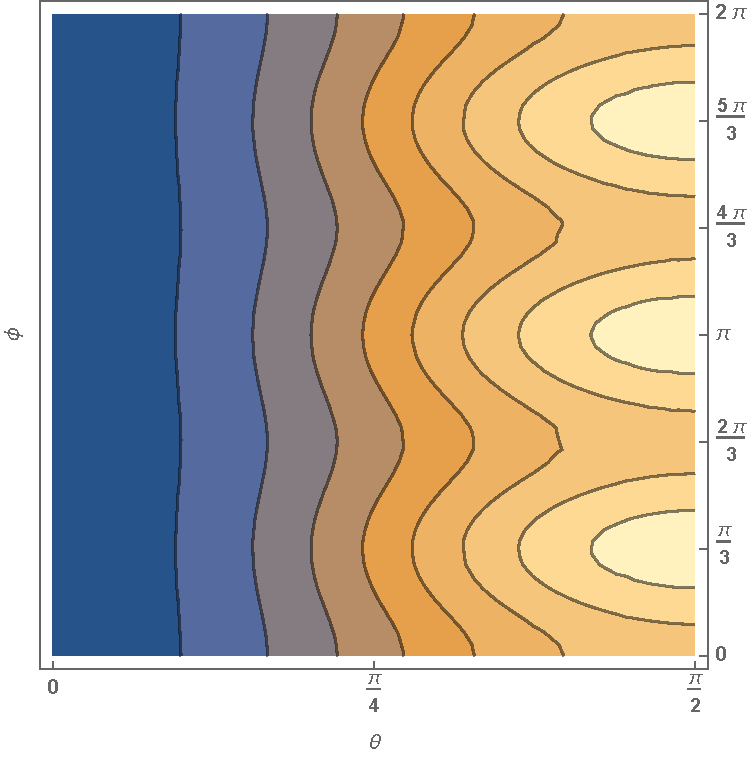
\includegraphics[width=0.60\linewidth]{potential.pdf}
	\caption{Potential surface for three identical particles. Symmetries due to translations and reflections are seen at $\phi = n\pi/3, \ (n = 1-5)$.}
	\label{fig:potential}
\end{figure*}

\section{Transformation of the Kinetic Energy Operator}\label{Appendix_2_2}
The kinetic energy operator of a particle with mass $\mu$ in a curvilinear coordinate system of $N$ dimensions is given by \cite{podolsky_1928}

\begin{equation}\label{eq:kinetic_e_op}
T = -\frac{1}{2\mu} \sum_{i=1}^{N} \sum_{j=1}^{N} \frac{1}{\sqrt{g}} \frac{\partial}{\partial q_i} \bigg(\sqrt{g} g^{ij} \frac{\partial}{\partial q_j}\bigg),
\end{equation}
where $g^{ij}$ is the inverse, or contravariant, metric tensor and $g$ is the determinant of the covariant metric tensor $g = \det(g_{ij}) \neq 0$. The metric tensor $g_{ij}$ describes the relationship between the set of curvilinear coordinates $\mathbf{q}$ and the set of regular Cartesian coordinates $\mathbf{x}$ through

\begin{equation}
g_{ij} = \sum_{\lambda = 1}^{N} \frac{\partial x_{\lambda}}{\partial q_{i}} \frac{\partial x_{\lambda}}{\partial q_{j}},
\end{equation}
where $x_{\lambda} = x_{\lambda}(q_1,\ldots,q_N)$. The metric is usefull for generalizing the concept of distance to general curvilinear coordinate frames and hence maintain the invariance of distance in different coordinate systems. Invariance of the square of the line element $d s^2$ under coordinate transformations can also be considered to define the metric itself since

\begin{equation}
d s^2 = d\mathbf{x} \cdot d\mathbf{x} = \sum_{i,j}^{N} g_{ij}  d q_{i} d q_{j} = g.
\end{equation}
Here the displacement differential vector is given by

\begin{equation}
d\mathbf{x} = \frac{\partial \mathbf{x}}{\partial q_{i}} d q_{i},
\end{equation} 
where $\mathbf{x}$ is the position vector.

The tranformation of interest for us is that from the mass weighted Jacobi coordinates $\mathbf{r}_k$ and $\mathbf{R}_k$ to a set of symmetric coordinates. Here we choose to work with one of the pair of the Jacobi coordinate sets $(i,j,k)=(1,2,3)$ and surpress the subscript $3$. Since the three-body system has $N=6$ dimensions after separating out the center-of-mass we collect the Cartesian components of the mass-weighted Jacobian vectors into the $6$-position

\begin{equation}
\mathbf{x} = 
\begin{pmatrix} 
\mathbf{r} \\
\mathbf{R} \\
\end{pmatrix} = 
\begin{pmatrix}
r_x \\
r_y \\
r_z \\
R_x \\
R_y \\
R_z\\
\end{pmatrix}.
\end{equation}

At any instant, three particles form a plane in $\mathbb{R}^3$. If we consider this plane to be the $xy$-plane -- and define the internal motion of the particles within this plane in terms of hyperspherical coordinates $(\rho, \Theta, \Phi)$ -- our coordinate system must rotate in this plane. That is, we use a body-fixed axis system $xyz$, which rotates with respect to the space-fixed axis system $x'y'z'$. The orientation of the body-fixed frame is related to the space-fixed frame by the Euler angles. With the $z$-axis perpendicular to the plane and with the positive axis in the direction of the vector $\mathbf{r} \times \mathbf{R}$, Smith and Whitten \cite{Smith_Whitten1968} defined these as   

\begin{equation}
\begin{aligned}
	r_x &= \rho \cos\Theta\cos\Phi,\\
	r_y &= -\rho \sin\Theta\sin\Phi,\\
	r_z &= 0\\
	R_x &= \rho \cos\Theta\sin\Phi,\\
	R_y &= \rho \sin\Theta\cos\Phi,\\
	R_z &= 0.
\end{aligned}   
\end{equation}

To describe how rotations of the body-fixed frame affects the derivatives in the space-fixed frame it is enough to consider infinitesimal rotations.  Let $d\mathbf{\Omega}$ be the angular displacement differential vector of the rotating axes $xyz$ with respect to the fixed axes $x'y'z'$

\begin{equation}
d\mathbf{\Omega} =
\begin{pmatrix}
d\Omega_x\\
d\Omega_y\\
d\Omega_z\\
\end{pmatrix}.
\end{equation}
Then the displacement differential vectors in the space-fixed frame transform like


\begin{subequations}
\begin{align}
	d{\mathbf{r}}' &= d\mathbf{r} + d\mathbf{\Omega} \times \mathbf{r},\\
	d{\mathbf{R}}' &= d\mathbf{R} + d\mathbf{\Omega} \times \mathbf{R},
\end{align}
\end{subequations}   
which is given explicitly by

\begin{align}
\begin{pmatrix}
d r'_x \\
d r'_y \\
d r'_z \\
d R'_x \\
d R'_y \\
d R'_z\\
\end{pmatrix} 
&= 
\begin{pmatrix*}[c]
\partial_{\rho} r_x & \partial_{\Theta} r_x & \partial_{\Theta} r_x & 0 & r_z & -r_y\\
\partial_{\rho} r_y & \partial_{\Theta} r_y & \partial_{\Theta} r_y & -r_z & 0 & r_x\\
\partial_{\rho} r_z & \partial_{\Theta} r_z & \partial_{\Theta} r_z & r_y & -r_x & 0\\
\partial_{\rho} R_x & \partial_{\Theta} R_x & \partial_{\Theta} R_x & 0 & R_z & -R_y\\
\partial_{\rho} R_y & \partial_{\Theta} R_y & \partial_{\Theta} R_y & -R_z & 0 & R_x\\
\partial_{\rho} R_z & \partial_{\Theta} R_z & \partial_{\Theta} R_z & R_y & -R_x & 0\\
\end{pmatrix*}
\begin{pmatrix}
d\rho\\
d\Theta\\
d\Phi\\
d\Omega_x\\
d\Omega_y\\
d\Omega_z\\
\end{pmatrix} \notag \\
&=
\begin{pmatrix*}[c]
\mathrm{cc} & \mathrm{-sc} & \mathrm{-cs} & 0 & 0 & \mathrm{ss}\\
\mathrm{-ss} & \mathrm{-cs} & \mathrm{-sc} & 0 & 0 & \mathrm{cc}\\
0 & 0 & 0 & \mathrm{-ss} & \mathrm{-cc} & 0\\
\mathrm{cs} & \mathrm{-ss} & \mathrm{cc} & 0 & 0 & \mathrm{-sc}\\
\mathrm{sc} & \mathrm{cc} & \mathrm{-ss} & 0 & 0 & \mathrm{cs}\\
0 & 0 & 0 & \mathrm{sc} & \mathrm{-cs} & 0\\
\end{pmatrix*}
\begin{pmatrix}
d\rho\\
\rho d\Theta\\
\rho d\Phi\\
\rho d\Omega_x\\
\rho d\Omega_y\\
\rho d\Omega_z\\
\end{pmatrix},\label{eq:matrix}
\end{align}
where the abbreviations are $\mathrm{cc} = \cos\Theta\cos\Phi$, $\mathrm{ss} = \sin\Theta\sin\Phi$, $\mathrm{cs} = \cos\Theta\sin\Phi$ and $\mathrm{sc} = \sin\Theta\cos\Phi$. In matrix notation \eqref{eq:matrix} may be expressed as

\begin{equation}
d\mathbf{x}' = \mathbf{A}d\mathbf{q},
\end{equation} 
in which      

\begin{equation}
d\mathbf{q} =
\begin{pmatrix}
d\rho\\
d\Theta\\
d\Phi\\
d\Omega_x\\
d\Omega_y\\
d\Omega_z\\
\end{pmatrix}.
\end{equation}
The squared line element $d s^2$ is then given by 

\begin{equation}
d s^2 = d\mathbf{x}' \cdot d\mathbf{x}' = d\mathbf{q}^{\mathrm{T}} \mathbf{A}^{\mathrm{T}} \mathbf{A}d\mathbf{q} = d\mathbf{q}^{\mathrm{T}} \mathbf{g} d\mathbf{q}.
\end{equation}
Here the metric tensor

\begin{equation}
\mathbf{g}=
\begin{pmatrix}
\mathbf{G} & \mathbf{C}\\
\mathbf{C}^\mathrm{T} & \mathbf{K}
\end{pmatrix}
\end{equation}
is partitioned into the submatrices $\mathbf{G}$, $\mathbf{K}$ and $\mathbf{C}$, which are given by 

\begin{align}
\mathbf{G} &=
\begin{pmatrix}
1 & 0      & 0\\
0 & \rho^2 & 0\\
0 & 0      & \rho^2
\end{pmatrix},\\
\mathbf{K} &=
\rho^2
\begin{pmatrix}
\sin^2\Theta & 0            & 0\\
0            & \cos^2\Theta & 0\\
0            & 0            & 1
\end{pmatrix},\\
\intertext{and}
\mathbf{C} &=
-\rho^2\sin^2(2\Theta)
\begin{pmatrix}
0 & 0 & 0\\
0 & 0 & 0\\
0 & 0 & 1
\end{pmatrix},
\end{align}
respectively. The inverse of the metric tensor $\mathbf{g}^{-1}$ is the given by

\begin{equation}
\mathbf{g}^{-1}=
\begin{pmatrix}
\mathbf{V} & \mathbf{W}\\
\mathbf{W}^\mathrm{T} & \mathbf{U}
\end{pmatrix},
\end{equation}
where the submatrices $\mathbf{V}$, $\mathbf{W}$ and $\mathbf{U}$ are given by

\begin{align}
\mathbf{V} &=
\begin{pmatrix}
1 & 0      & 0\\
0 & 1/\rho^2 & 0\\
0 & 0      & 1/\rho^2\cos^2(2\Theta)
\end{pmatrix},\\
\mathbf{U} &=
\frac{1}{\rho^2}
\begin{pmatrix}
1/\sin^2\Theta & 0            & 0\\
0            & 1/\cos^2\Theta & 0\\
0            & 0            & 1/\cos^2(2\Theta)
\end{pmatrix},\\
\intertext{and}
\mathbf{W} &=
\frac{\sin(2\Theta)}{\rho^2\cos^2(2\Theta)}
\begin{pmatrix}
0 & 0 & 0\\
0 & 0 & 0\\
0 & 0 & 1
\end{pmatrix},
\end{align}
respectively. The determinant of the metric tensor is then

\begin{align}
g &=
\mid\mathbf{g}\mid=
\begin{vmatrix}
\mathbf{G} & \mathbf{C}\\
\mathbf{C}^T & \mathbf{K}
\end{vmatrix}
=
\begin{vmatrix}
\mathbf{G} & \mathbf{C}\\
0 & \mathbf{K} - \mathbf{C}^T \mathbf{G}^{-1} \mathbf{C}
\end{vmatrix}\\
&=
\mid \mathbf{G} \mid \cdot \mid\mathbf{K} - \mathbf{C}^T \mathbf{G}^{-1} \mathbf{C} \mid
=
\frac{\rho^{10}}{16}\sin^2(4\Theta)
\end{align}
and subsequently the square root of the metric reads
\begin{equation}
\sqrt{g}=\frac{\rho^5}{4}\sin(4\Theta).
\end{equation}
Now, if the momentum vector is given by

\begin{equation}
\mathbf{p} = i 
\begin{pmatrix}
\partial/\partial q_1\\
\vdots\\
\partial/\partial q_N\\
\end{pmatrix}
\end{equation}
we can express the kinetic energy operator given in \eqref{eq:kinetic_e_op} in terms of this vector and the metric

\begin{equation}\label{eq:T_SW}
\begin{aligned}
-T &= -\frac{1}{2\mu \sqrt{g}} \mathbf{p}^\mathrm{T} \sqrt{g} \mathbf{g}^{-1} \mathbf{p}\\
&= \frac{1}{2\mu \rho^5 \sin(4\Theta)}\Bigg[ \frac{\partial}{\partial \rho} \Bigg(\rho^5 \sin(4 \Theta) \frac{\partial}{\partial \rho}\Bigg) + \frac{\partial}{\partial \Theta}\Bigg(\rho^3\sin(4\Theta)\frac{\partial}{\partial\Theta}\Bigg)\\ &+\frac{\partial}{\partial\Phi}\Bigg(2\rho^3\tan(2\Theta)\frac{\partial}{\partial\Phi} + 2\tan^2(2\Theta)\cos(2\Theta)\frac{\partial}{\partial\Omega_z}\Bigg)\\
&+\frac{\partial}{\partial\Omega_x}\Bigg(4\rho^3\cot(\Theta)\cos(2\Theta)\frac{\partial}{\partial\Omega_x}\Bigg)\\
&+\frac{\partial}{\partial\Omega_y}\Bigg(4\rho^3\tan(2\Theta)\cos(2\Theta)\frac{\partial}{\partial\Omega_y}\Bigg)\\
&+\frac{\partial}{\partial\Omega_z}\Bigg(2\rho^3\tan^2(2\Theta)\frac{\partial}{\partial\Phi}+2\rho^3\tan(2\Theta)\frac{\partial}{\partial\Omega_z}\Bigg)\Bigg]\\
&=\frac{1}{2\mu}\Bigg[\frac{1}{\rho^5}\frac{\partial}{\partial\rho}\Bigg(\rho^5\frac{\partial}{\partial\rho}\Bigg) + \frac{1}{\rho^2\sin(4\Theta)}\frac{\partial}{\partial\Theta}\Bigg(\sin(4\Theta)\frac{\partial}{\partial\Theta}\Bigg)\\
&+\frac{1}{\rho^2\cos^2(2\Theta)}\frac{\partial^2}{\partial\Phi^2} + \frac{\sin(2\Theta)}{\rho^2\cos^2(2\Theta)}\frac{\partial}{\partial\Phi}\frac{\partial}{\partial\Omega_z}\\
&+\frac{1}{\rho^2\sin^2(\Theta)}\frac{\partial^2}{\partial\Omega^2_x} + \frac{1}{\rho^2\cos^2(\Theta)}\frac{\partial^2}{\partial\Omega^2_y} + \frac{\sin(2\Theta)}{\rho^2\cos^2(2\Theta)}\frac{\partial}{\partial\Omega_z}\frac{\partial}{\partial\Phi}\\
&+ \frac{1}{\rho^2\cos^2(2\Theta)}\frac{\partial^2}{\partial\Omega^2_z}\Bigg]\\
&=\frac{1}{2\mu\rho^5}\frac{\partial}{\partial\rho}\Bigg(\rho^5\frac{\partial}{\partial\rho}\Bigg) + \frac{1}{2\mu\rho^2}\Bigg[\frac{1}{\sin(4\Theta)}\frac{\partial}{\partial\Theta}\Bigg(\sin(4\Theta)\frac{\partial}{\partial\Theta}\Bigg)\\
&+\frac{1}{\cos^2(2\Theta)}\frac{\partial^2}{\partial\Phi^2} \Bigg]+\frac{1}{2\mu\rho^2}\Bigg[\frac{1}{\sin^2(\Theta)}\frac{\partial^2}{\partial\Omega^2_x} + \frac{1}{\cos^2(\Theta)}\frac{\partial^2}{\partial\Omega^2_y} + \frac{1}{\cos^2(2\Theta)}\frac{\partial^2}{\partial\Omega^2_z}\\
&+ \frac{2\sin(2\Theta)}{\cos^2(2\Theta)}\frac{\partial}{\partial\Phi}\frac{\partial}{\partial\Omega_z}\Bigg].
\end{aligned}
\end{equation}

Now, as have been mentioned previously, we use the Euler angles $\alpha,\beta,\gamma$ to relate the body-fixed axes $xyz$ with the space-fixed axes $x'y'z'$. Any coordinate frame that coincide with the space-fixed frame can be made to coincide with the body-fixed frame by performing a series of three basic rotations (right-handed). There are several ways for defining the Euler angles, the convention used by Johnson \cite{Johnson_1983} is adopted here and the method is decribed in detail in \cite{arfken_weber_harris_2013}. If the line of nodes $\xi$ are the intersection of the planes $x'y'$ and $xy$, then $\alpha$ is the angle between the $y'$-axis and the line of nodes. The operational sequence are the following:

\begin{enumerate}[(i)]  
	\item First rotate the coordinates $x'y'z'$ counterclockwise through an angle $\alpha$ in the range $0 \leq \alpha < 2\pi$ about the $z'$-axis, using $\mathbf{S}_{\alpha}$, into the new coordinates $\bar{x}'\xi z'$.
	\item Then rotate the coordinates $\bar{x}' \xi z'$ counterclockwise through an angle $\beta$ $(0 \leq \beta \leq \pi)$ about the line of nodes, using $\mathbf{S}_{\beta}$, into the new coordinates $\bar{x} \xi z$.
	\item Finally rotate the coordinates $\bar{x} \xi z$ counterclockwise by an angle $\gamma$ $(0 \leq \gamma < 2\pi)$ about the $z$-axis (the former $z'$-axis) using $\mathbf{S}_{\gamma}$, into the body-fixed coordinates $xyz$.
\end{enumerate}   
The total rotation matrix is then the triple matrix product of the basic rotation matrices $\mathbf{S} = \mathbf{S}_{\alpha}\mathbf{S}_{\beta}\mathbf{S}_{\gamma}$, in which

\begin{equation}
\mathbf{S}_{\alpha}=
\begin{pmatrix}
\cos\alpha & \sin\alpha  & 0\\
-\sin\alpha & \cos\alpha & 0\\
0            & 0            & 1
\end{pmatrix},\\
\end{equation}

\begin{equation}
\mathbf{S}_{\beta}=
\begin{pmatrix}
\cos\beta & 0  & -\sin\beta\\
0 & 1 & 0\\
\sin\beta & 0  & \cos\beta
\end{pmatrix},\\
\end{equation}

\begin{equation}
\mathbf{S}_{\gamma}=
\begin{pmatrix}
\cos\gamma & \sin\gamma  & 0\\
-\sin\gamma & \cos\gamma & 0\\
0            & 0            & 1
\end{pmatrix},\\
\end{equation}
and

\begin{equation}
\mathbf{S}=
\begin{pmatrix}
\cos\gamma \cos\beta \cos\alpha -\sin\gamma \sin\alpha & \cos\gamma \cos\beta \sin\alpha \sin\gamma \cos\alpha  & -\cos\gamma \sin\beta\\
-\sin\gamma \cos\beta \cos\alpha -\cos\gamma \sin\alpha & \sin\gamma \cos\beta \sin\alpha +\cos\gamma \cos\alpha & \sin\gamma \sin\beta\\
\sin\beta \cos\alpha & \sin\beta \sin\alpha & \cos\beta
\end{pmatrix}.
\end{equation}
The cartesian coordinates $\mathbf{x}$ and $\mathbf{x}'$ of a point $P$ in the two frames are thus related through

\begin{equation}
\mathbf{x} = \mathbf{S}\mathbf{x}'. 
\end{equation}
Now, the general angular displacement differential  $d\mathbf{\Omega}$ can be considered as consisting of three consecutive infinitesimal rotations where $d\Omega_{\alpha} = d\alpha$, $d\Omega_{\beta} = d\beta$ and $d\Omega_{\gamma} = d\gamma$. The vector $d\mathbf{\Omega}$ can be obtained as the sum of three different angular displacement differential vectors; $d\mathbf{\Omega_{\alpha}}$ is along the space-fixed $z'$-axis, $d\mathbf{\Omega_{\beta}}$ is along the line of nodes and $d\mathbf{\Omega_{\gamma}}$ is along the body-fixed $z$-axis \cite{goldstein_poole_safko_2000}. Since $d\mathbf{\Omega_{\alpha}}$ is along the $z'$-axis, its components are obtained by the applying the total rotation matrix. Thus, if the total rotation matrix is written

\begin{equation}
\mathbf{S} = [\mathbf{S}_1 \quad \mathbf{S}_2 \quad \mathbf{S}_3],
\end{equation}
then the body-fixed displacement differential angles $d\mathbf{\Omega}_{\alpha}$ are related to the Euler angles through

\begin{equation}
(\mathbf{\Omega}_{\alpha})_{\mathbf{x}} = \mathbf{S}_3 d\alpha= 
\begin{pmatrix}
-\sin\beta \cos\gamma \\
\sin\beta \sin\gamma \\
\cos\beta
\end{pmatrix} d\alpha.
\end{equation}
Next, because $d\mathbf{\Omega_{\beta}}$ is along the line of nodes, we only need to apply the last transformation $\mathbf{S}_{\gamma}$ to retreive

\begin{equation}
(\mathbf{\Omega}_{\beta})_{\mathbf{x}} = \mathbf{S}_{\gamma_2} d\beta= 
\begin{pmatrix}
\sin\gamma \\
\cos\gamma \\
0
\end{pmatrix} d\beta.
\end{equation}
No transformation is needed for $d\mathbf{\Omega_{\gamma}}$ since it is already directed along the body-fixed $z$-axis. The transformations are finally summarized into the total transformation matrix, which relates the body-fixed infinitesimal rotations to the Euler angles through

\begin{equation}
\begin{pmatrix}
d\Omega_x\\
d\Omega_y\\
d\Omega_z
\end{pmatrix}
=
\tilde{\mathbf{S}}\begin{pmatrix}
d\alpha\\
d\beta\\
d\gamma
\end{pmatrix},
\end{equation}
where

\begin{equation}\label{eq:S_matrix}
\tilde{\mathbf{S}}=
\begin{pmatrix}
-\sin\beta\cos\gamma & \sin\gamma & 0\\
\sin\beta\sin\gamma  & \cos\gamma & 0\\
\cos\beta 			 & 0          & 1
\end{pmatrix}.
\end{equation}
Thus, a transformation of coordinates

\begin{equation}
d\mathbf{q} =
\begin{pmatrix}
d\rho\\
d\Theta\\
d\Phi\\
d\Omega_x\\
d\Omega_y\\
d\Omega_z\\
\end{pmatrix}
\longrightarrow
d\mathbf{q}' =
\begin{pmatrix}
d\rho\\
d\Theta\\
d\Phi\\
d\alpha\\
d\beta\\
d\gamma\\
\end{pmatrix}
\end{equation}
correspond to a transformation of the metric, which is easily derived from the squared line element, where

\begin{equation}
d s^2 = d \mathbf{q}^{\mathrm{T}}\mathbf{g}d \mathbf{q} = (d \mathbf{q}')^\mathrm{T}\mathbf{g}'d\mathbf{q}'.
\end{equation}
The metric thus transform as 

\begin{equation}
\mathbf{g}'=\mathbf{B}^{\mathrm{T}}\mathbf{g}\mathbf{B},
\end{equation}
in which

\begin{equation}
\mathbf{B} = 
\begin{pmatrix}
\mathbf{I} & 0\\
0      & \tilde{\mathbf{S}}
\end{pmatrix}.
\end{equation}
Subsequently, the square root of the determinant transform into

\begin{equation}
g'^{1/2}=(\mid\mathbf{B}\mid^2 \mid\mathbf{g}\mid)^{1/2} = (\mid\tilde{\mathbf{S}}\mid^2 \mid\mathbf{g}\mid)^{1/2}
= \frac{\rho^5}{4}\sin(4\Theta)\sin\beta.
\end{equation}
Since a general curvilinear coordinate system of $N$ dimensions have a volume element

\begin{equation}
d ^Nv = g^{1/2}\prod_{i=1}^{N} d q_i,
\end{equation}
the sought volume element is  

\begin{equation}
d^6v = g^{1/2}\prod_{i=1}^{6} d q_i = \frac{\rho^5}{4}\sin(4\Theta)\sin\beta d\rho d\Theta d\Phi d\alpha d\beta d\gamma.
\end{equation}
Lastly, to produce a representation of the entire internal configuration
space that is unbiased by the particular choice of the three Jacobi coordinate sets, we follow Kuppermann's mapping procedure \cite{KUPPERMANN1975374} and make the following modification of the internal angles

\begin{equation}
\begin{aligned}
\Theta &= \frac{\pi}{4}-\frac{\theta}{2} \implies \frac{\partial}{\partial\Theta} = -2\frac{\partial}{\partial\theta},\\
\Phi &= \frac{\pi}{4}-\frac{\phi}{2} \implies \frac{\partial}{\partial\Phi} = -2\frac{\partial}{\partial\phi}.
\end{aligned}
\end{equation}
Now, define

\begin{equation}
\mathbf{P} = 
-i
\begin{pmatrix}
\partial/\partial\rho\\
\partial/\partial\theta\\
\partial/\partial\phi
\end{pmatrix}
=
\begin{pmatrix}
P_{\rho}\\
P_{\theta}\\
P_{\phi}
\end{pmatrix}
\end{equation}
and

\begin{equation}\label{eq:J_vector}
\mathbf{J} = 
-i
\begin{pmatrix}
\partial/\partial\Omega_x\\
\partial/\partial\Omega_y\\
\partial/\partial\Omega_z
\end{pmatrix}
=
\begin{pmatrix}
J_x\\
J_y\\
J_z
\end{pmatrix},
\end{equation}
where the operators $J_x$, $J_y$ , and $J_z$ are the total angular momentum operators in the body-fixed frame, which can be expressed in terms of the Euler angle coordinates by the relation

\begin{equation}
\begin{pmatrix}
J_x\\
J_y\\
J_z
\end{pmatrix} =
\begin{pmatrix}
-\cos\gamma/\sin\beta & \sin\gamma & \cot\beta \cos\gamma\\
\sin\gamma/\sin\beta & \cos\gamma & -\cot\beta \sin\gamma\\
0 & 0 & 1
\end{pmatrix}
\begin{pmatrix}
P_{\alpha}\\
P_{\beta}\\
P_{\gamma}
\end{pmatrix}.
\end{equation} 
This can be shown using the chain rule for partial differentiation

\begin{equation}
P_{\sigma} = \sum_{\lambda} \frac{\partial \Omega_{\lambda}}{\partial \sigma} J_{\lambda},
\end{equation}
where $\sigma = (\alpha,\beta,\gamma)$ and $\lambda = (x,y,z)$. The partial derivatives are calculated using the inverse of \eqref{eq:S_matrix}

\begin{equation}\label{eq:S_matrix}
\tilde{\mathbf{S}}^{-1}=
\begin{pmatrix}
-\cos\gamma/\sin\beta & \sin\gamma/\sin\beta & 0\\
\sin\gamma  & \cos\gamma & 0\\
\cot\beta \cos\gamma  & -\cot\beta \sin\gamma  & 1
\end{pmatrix}.
\end{equation}
Now, using the relations

\begin{equation}
\begin{aligned}
&\sin 4\Theta   =\sin 2\theta\\
&\cos^2 2\Theta =\sin^2 \theta\\
&\sin^2 2\Theta =\cos^2 \theta\\
&\cos^2\Theta    =\frac{1}{2}(1+\sin\theta)\\
&\sin^2\Theta    =\frac{1}{2}(1-\sin\theta)
\end{aligned}
\end{equation}
in conjunction with \eqref{eq:J_vector} the kinetic energy operator \eqref{eq:T_SW} becomes

\begin{equation}
\begin{aligned}
T &=-\frac{\hbar^2}{2\mu}\Bigg[\frac{1}{\rho^5}\frac{\partial}{\partial\rho}\rho^5\frac{\partial}{\partial\rho} + \frac{4}{\rho^2}\Bigg(\frac{1}{\sin(2\theta)}\frac{\partial}{\partial\theta}\sin(2\theta)\frac{\partial}{\partial\theta}\\
&+\frac{1}{\sin^2(\theta)}\frac{\partial^2}{\partial\phi^2} \Bigg)\Bigg]-\frac{1}{\mu\rho^2}\Bigg[\frac{J^2_x}{(1-\sin\theta)} + \frac{J^2_y}{(1+\sin\theta)} +\frac{J^2_z}{2\sin^2\theta}\Bigg]\\
&+ \frac{4i\hbar\cos\theta J_z}{2\mu\rho^2\sin^2\theta}\frac{\partial}{\partial\phi},
\end{aligned}
\end{equation}
with the corresponding volume element

\begin{equation}
d^6 v = \frac{1}{8}\rho^5 \sin\theta\cos\theta\sin\beta d\rho d\theta d\phi d\alpha d\beta d\gamma.
\end{equation}
If we only consider $J=0$ states, the Hamiltonian reduces to 

\begin{equation}
H_{0} = -\frac{1}{2 \mu} \Bigg[ \frac{1}{\rho^{5}} \frac{\partial}{\partial \rho} \rho^{5} \frac{\partial}{\partial \rho} + \frac{4}{\rho^{2}}\Big( \frac{1}{\sin(2\theta)} \frac{\partial}{\partial \theta} \sin(2\theta) \frac{\partial}{\partial \theta} + \frac{1}{\sin^{2}(\theta)} \frac{\partial^{2}}{\partial \phi^{2}} \Big) \Bigg] + V(\rho, \theta, \phi).
\end{equation}
By rescaling the wave function $\psi = \rho^{5/2} \Psi$ the Schr{\"o}dinger equation becomes

\begin{equation}
H \psi = E \psi,
\end{equation}
where the transformed Hamiltonian operator is given by

\begin{equation}
H = \rho^{5/2}H_{0} \rho^{-5/2}. 
\end{equation}
This transformation removes the first derivative in the hyper radial kinetic-energy operator and we get the final expression for the Hamiltonian

\begin{align}
H &= -\frac{\hbar^{2}}{2 \mu} \Bigg[ -\frac{15}{4} \frac{1}{\rho^{2}} + \frac{\partial^{2}}{\partial \rho^{2}}+ \frac{4}{\rho^{2}}\Big( \frac{1}{\sin(2\theta)} \frac{\partial}{\partial \theta} \sin(2\theta) \frac{\partial}{\partial \theta} + \frac{1}{\sin^{2}(\theta)} \frac{\partial^{2}}{\partial \phi^{2}} \Big) \Bigg] + V(\rho, \theta, \phi)\\
&= -\frac{\hbar^{2}}{2 \mu}\frac{\partial^2}{\partial \rho^2} + \frac{\hbar^{2}}{2 \mu \rho^{2} } \Bigg(\Lambda^2 + \frac{15}{4}\Bigg)+ V(\rho, \theta, \phi),
\end{align}
where $\Lambda^2$ is the grand angular momentum operator.